%!TEX root = ../thesis.tex

\chapter{Eigener Ansatz: Social Online Community Connectors (SOCC)} % (fold)
\label{cha:eigener_ansatz_social_online_community_connectors_socc_}

Aufbauend auf den in Kapitel \ref{cha:analyse} identifizierten Komponenten und Wahl der für ein System zur Synchronisation von Beiträgen passenden Techniken, soll nun der als \emph{Social Online Community Connectors} (SOCC) benannter Ansatz vorgestellt werden. SOCC setzt für seine Aufgabe auf Techniken des in den Grundlagenkapitel beschriebenen Semantic Webs. Der Einsatz von offenen Datenformaten wie RDF und den darauf aufbauenden FOAF und SIOC nicht nur für den hier beschrieben Zweck sondern auch für andere Projekte verwendet werden kann. 

Der Aufbau von SOCC zeig die Abbildung \ref{fig:uebersicht_socc}. Ein \emph{Connector} des SOCC dient als Verbindungselement zwischen zwei oder mehr Webseiten, die unter dem Begriff \emph{Social Online Community} (SOC)zusammengefasst werden. Also einer Gemeinschaft die im Web auf soziale Weise Wissen austauscht. SOCC stützt sich dabei dabei auf die Prinzipien für die Verbindung von Daten im Web von Tim Berners-Lee \cite{Berners-Lee2009}:

\begin{description}
    \item[\enquote{Use URIs as names for things}] Seiten, Foren, Threads und Beiträge sollten immer über eine URI benannt werden, so das andere Anwendungen diese verwenden können.

    \item[\enquote{Use HTTP URIs so that people can look up those names}] Die verwendeten URIs sollten dereferenzierbar sein, um auf die dahinter liegenden Daten zugreifen zu können.

    \item[\enquote{When someone looks up a URI, provide useful information, using the standards (RDF*, SPARQL)}] Die Daten sollten in einen Standard für das Semantic Web formatiert werden. Wie schon wähnt setzt SOCC dazu auf RDF und darauf aufbauenden Ontologien wie FOAF und SIOC. Dadurch können zum Beispiel andere Anwendungen mit Anfragen in SPARQL\footnote{\url{http://www.w3.org/TR/sparql11-overview}} nach Beiträgen suchen.

    \item[\enquote{Include links to other URIs. so that they can discover more things.}] Nicht nur die Struktur eine Diskussion kann über Links verfolgt werden, auch das Gewinnen zusätzlicher Informationen ist so möglich. Beiträge können auf Lernmaterialien wie Folien oder Videos verweisen oder über das FOAF-Profil eines Autor können weitere Beiträge von ihm gefunden werden. 
\end{description}

URIs sind also das wichtigste Element mit denen SOCC arbeitet. Soll zum Beispiel eine Diskussion synchronisiert werden, muss einem Connector die URI übergeben werden, hinter der sich die Daten befinden. Ein Connector ist nur für eine einzige SOC zuständig. Aber eine  SOC kann über mehrere Connectoren angesprochen werden, wodurch eine Arbeitsteilung möglich ist.

\begin{figure}[ht]
    \centering
    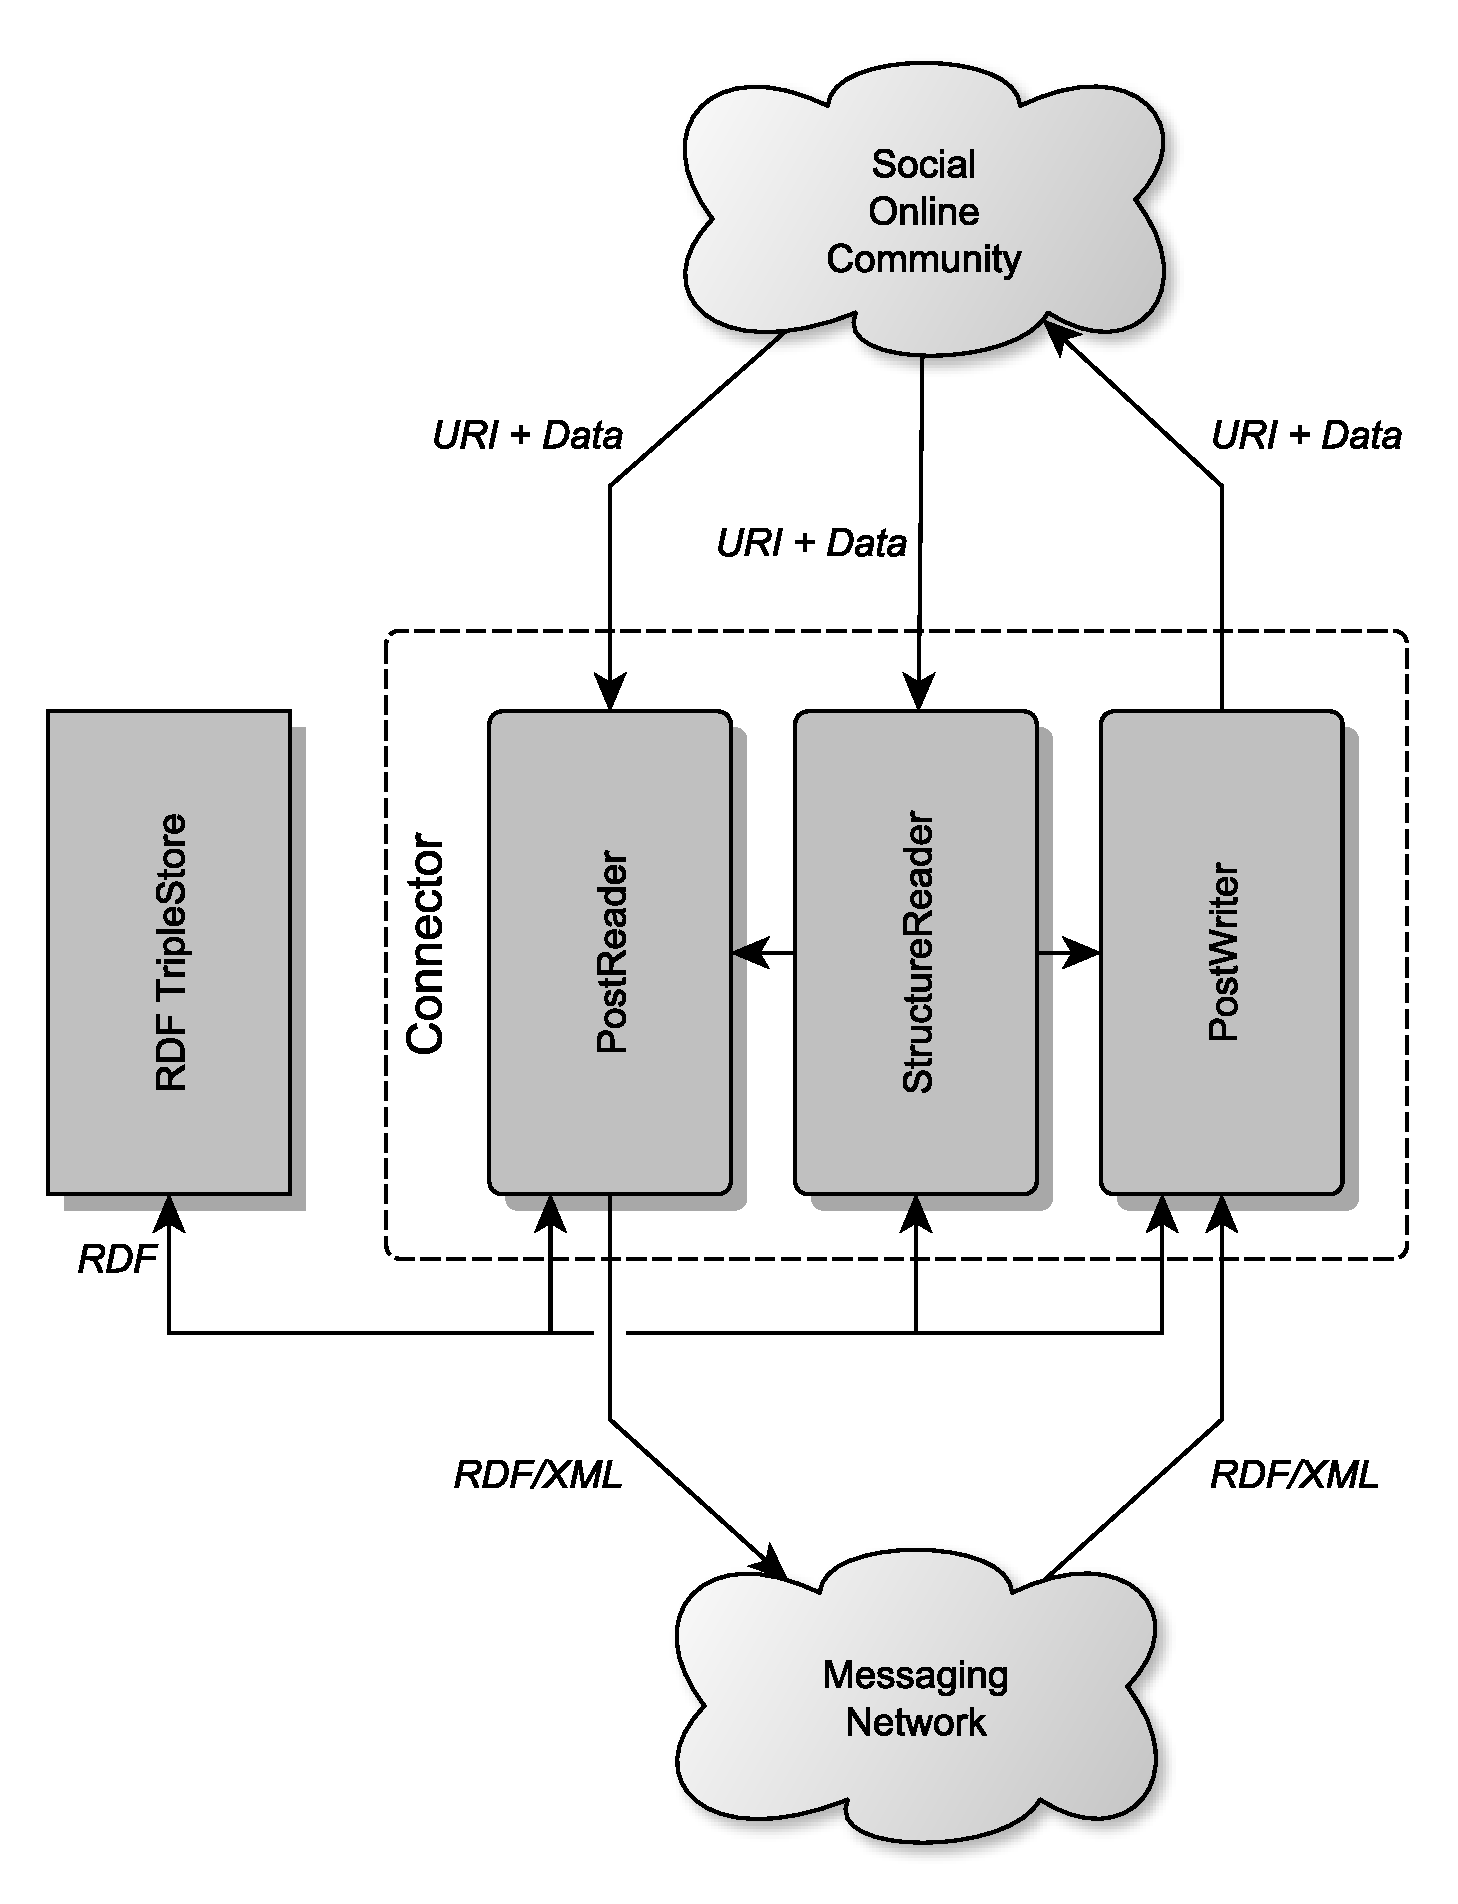
\includegraphics[
        width=0.5\textwidth,
        keepaspectratio=true]
    {assets/images/socc_connector_overview}
    \caption{Übersicht der Komponenten der SOCC}
    \label{fig:uebersicht_socc}
\end{figure}


Intern besteht ein Connector aus drei Teilkomponenten die zum Einen für das Lesen (\emph{PostReader}) und Schreiben (\emph{PostWriter}) von Beiträgen verwendet werden, zum Andren aus einen \emph{StructureReader} der für das auslesen der Struktur der einzelnen Diskussionen verantwortlich ist. Eine genaue Beschreibung dieser Komponenten folgt in Abschnitt \ref{sec:design_eines_connectors}.

Jeder Connector hat Zugriff auf eine als \emph{Triplestore} bezeichnete Datenbank in der RDF-Triple gespeichert und unter anderen mit SPARQL abgefragt werden. Der Connector benutzt diesen Triplesore als Speicher in dem seine Konfigurationsdaten lagern, aber auch zusätzliche Daten die er von Außerhalb, wie eine Liste von Benutzerkonten, benötigt. Er wird aber auch benutzt um Daten zu speichern die während des Betriebes anfallen, da sie so irgendwann wieder verwendet werden können ohne sie erneut zusammenzusuchen. Zum Beispiel die Daten über die Struktur der verwendeten SOC.

Die Beiträge werden dann zwischen den einzelnen Connectoren über ein Nachrichtennetzwerk auf der Basis von Apache Camel ausgetauscht. Die Beschreibung dieser als \emph{SOCC-Camel} bezeichneten Komponnente geschieht in Kapitel \ref{sec:socc_camel}.

\section{Datenformat} % (fold)
\label{sec:datenformat}

\todo[inline]{Auch begründen warum die Verwendung von Ontologien und nicht bspw. die Entwicklung eines XML Schemas (alternativ bei der Analyse Kap. 3.2)}

% section datenformat (end)

\section{Konfiguration} % (fold)
\label{sec:konfiguration}

Dass ein Connector funktionieren kann, muss er von außen mit Informationen zugeführt bekommen welche er zum Betrieb braucht. Die sind zum Beispiel Informationen zu Benutzerkonten oder Parameter für die verwendete API. Da einige dieser Informationen werden nicht nur von einen Connector benutzt werden, ist es sinnvoll diese zusammen an einen Ort zu speichern und wiederverwenden zu können. Die wichtigsten Informationen für die Konfiguration der Connectoren stellen die Benutzerkonten dar. Sie enthalten unter anderem die Informationen um Zugriff auf die einzelnen APIs zu erhalten. Da die Benutzerkonten wie im Abschnitt \ref{sec:datenformat} beschrieben im FOAF Format in einen Triplestore gespeichert werden, stellt es sich als Vorteil heraus die übrigen Informationen ebenfalls dort zu speichern und mit den schon vorhandenen zu verbinden. 

Aus diesem Grund wurde für Konfiguration eines Connectors die \emph{Connector Config Ontology} entwickelt. Diese Ontologie ist sehr einfach gehalten und baut auf schon vorhandenen Ontologien auf. Zusätzlich musste die SIOC Ontologie so erweitert werden, dass die Integration von Autorisierungs- und Authentifizierungsinformationen möglich war. 

\subsection{SOCC Connector Config Ontologie} % (fold)
\label{sub:connector_config_ontologie}

Abbildung \ref{fig:uebersicht_conector_cfg} zeigt die entwickelte \emph{SOCC Connector Config} Ontologie. Sie besteht aus einer einzigen Klasse \texttt{ConnectorConfig} und fünf Eigenschaften für diese.
\todo[inline]{Einleitung umschreiben, klingt scheiße}

\begin{figure}[ht]
    \centering
    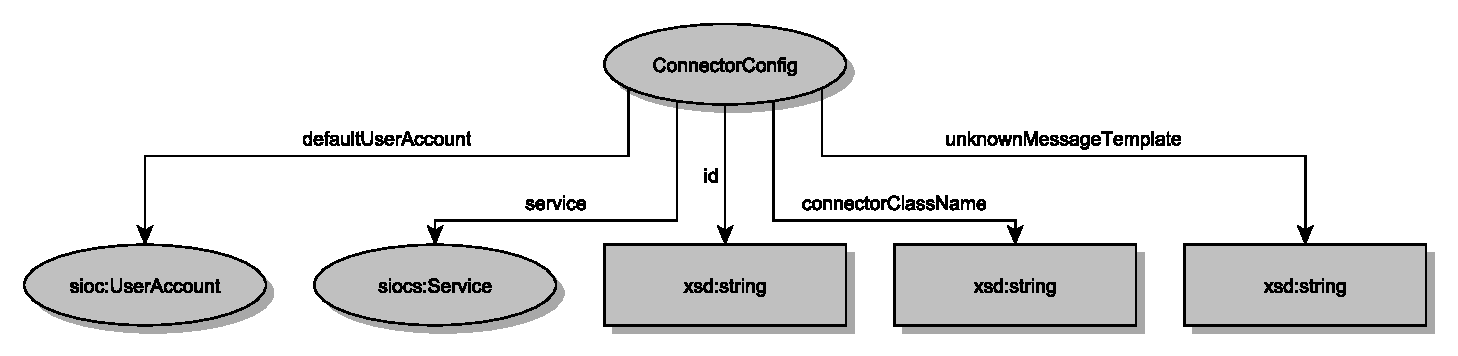
\includegraphics[
        width=\textwidth,
        keepaspectratio=true
    ]{assets/images/connector_config_ontology}
    \caption{Schema der SOCC Connector Config Ontology}
    \label{fig:uebersicht_conector_cfg}
\end{figure}

Jeder Connector erhält einen eindeutigen \texttt{id} zugewiesen, um jeden Connectoren später eindeutig identifizieren zu können. Die Eigenschaft \texttt{connectorClassName} beschreibt den vollständigen Klassennamen des beschriebenen Connector. Diese wird für das laden der richtigen Implementierung benötigt. Manchmal kann es passieren, dass keine passendes Benutzerkonto zum Weiterleiten eins Beitrags gefunden werden kann. Dadurch es es wünschenswert solche Beiträte dahingegen zu verändern, dass eine Verweis auf den original Autor und vielleicht wo der Beitrag gemacht wurde vorhanden ist. Durch die Eigenschaft \texttt{unknownMessageTemplate} kann eine Vorlage für das Aussehen des des Verweises definiert werden.Innerhalb dieser Vorlage stehen einige Variablen in der Form \enquote{\texttt{\{varName\}}} zur Verfügung. Alle zur Zeit vorhandenen Variablennamen und deren Ersetzung sind in Tabelle \ref{tbl:unknown_message_template_vars} zu sehen. 

\begin{table}[ht]
    \caption{Variablennamen und Ersetzung innerhalb von \texttt{unknownMessageTemplate} }
    \centering
    \begin{tabular}{r|l}
        \textbf{varName} & \textbf{Ersetzt durch} \\
        \hline
        \texttt{message} & Original Beitrag \\
        \texttt{sourceUri} & URI des original Beitrags \\
        \texttt{connectorId}  & ID des aktuellen Connectors \\
        \texttt{serviceName}  & Name des vom Connector verwendeten Service \\
        \texttt{creationDate} & Erstelldatum des Beitrags (falls bekannt) \\
        \texttt{authorName}   & Name des Autors (falls bekannt)          
    \end{tabular}
    \label{tbl:unknown_message_template_vars}
\end{table}

Für die Nutzung einiger APIs müssen bestimmte Parameter angegeben werden. Dies könnte zum Beispiel die genau Adresse des Dienstes sein. Hierzu wird auf die schon Bestehende SIOC Services Ontologie zurückgegriffen. Diese stellt eine Klasse \emph{Service} zur Verfügung und mittels der Eigenschaft \texttt{service} kann ein solcher Service einem Connector zugewiesen werden. Der genaue Aufbau eines solchen Services wird im Abschnitt \ref{sub:services} dargestellt. Die letzte Information für die Konfiguration eins Connectors ist eine vordefinierter Benutzer (im Folgenden Defaultuser genannt) und wird mit der Eigenschaft \texttt{defaultUserAccount} festgelegt. Dieser Defaultuser erfüllt im Großen und Ganzen zwei Aufgaben. Als Erstes wird er für lesende Zugriffe der API auf den verwendeten Dienst genutzt. Hierzu ist ein einzelnes Benutzerkonto vollkommen ausreichend, da nur die gelesenen Daten wichtig sind und nicht von welchen Konto sie kommen.Die zweite Aufgabe bezieht sich auf das stellvertretende Schreiben einzelner Benutzer. Nicht immer werden die dazu notwendigen Daten von den Benutzer zur Verfügung gestellt oder sind unbekannt. In diesem Fall wird der Defaultuser genutzt und der Beitrag mit einem Vermerk zum original Autor über diesen geschrieben.

% subsubsection connector_config_ontology (end)

\subsection{Services} % (fold)
\label{sub:services}

Wie eben schon beschrieben, existiert für SIOC ein Modul zur einfachen Modellierung von Diensten auf semantischer Ebene: Das SIOC Services Module (Präfix \emph{siocs:}). Kernstück dieses Moduls ist die Klasse Service, wie auf Abbildung \ref{fig:uebersicht_sioc_services} zu sehen ist. Mit dieser Klasse kann durch eine Hand voll Eigenschaften ein Dienst beschrieben werden. Für diese Arbeit ist davon die wichtigste Eigenschaft \texttt{service\_endpoint}. Durch diese kann die Adresse festgelegt werden, unter dem ein bestimmter Dienst erreichbar ist. Gerade bei Plattformen die nicht an eine feste Adresse (Foren, Blogs, $\dots$) gebunden sind, ist diese Angabe unerlässlich. Die Eigenschaften \texttt{has\_service} und \texttt{service\_of} sind sind ideal zur Verbindung von einzelnen SIOC UserAccounts mit einem Service. Diese Verbindung hilft dabei für das stellvertretende Schreiben von Beiträgen schnell die passenden Benutzerdaten zu finden. Ebenfalls nützlich ist \texttt{max\_results}. Manche Dienste erlauben es nur eine maximale Anzahl an Ergebnissen pro Aufruf zurückgeben zu lassen. Da sich diese Anzahl über die Zeit ändern kann ist es nicht sinnvoll diese fest im Programm festzulegen, kann diese so im Nachhinein verändert werden. Für SOCC weniger interessant aber Vollständigkeit halber seien noch erwähnt \texttt{service\_protocol} zum Angeben des verwendeten Übertragungsprotokolls REST, SOAP, $\dots$) und \texttt{service\_definition} mit dem auf eine weiterführende Definition verwiesen werden kann. 

\begin{figure}[ht]
    \centering
    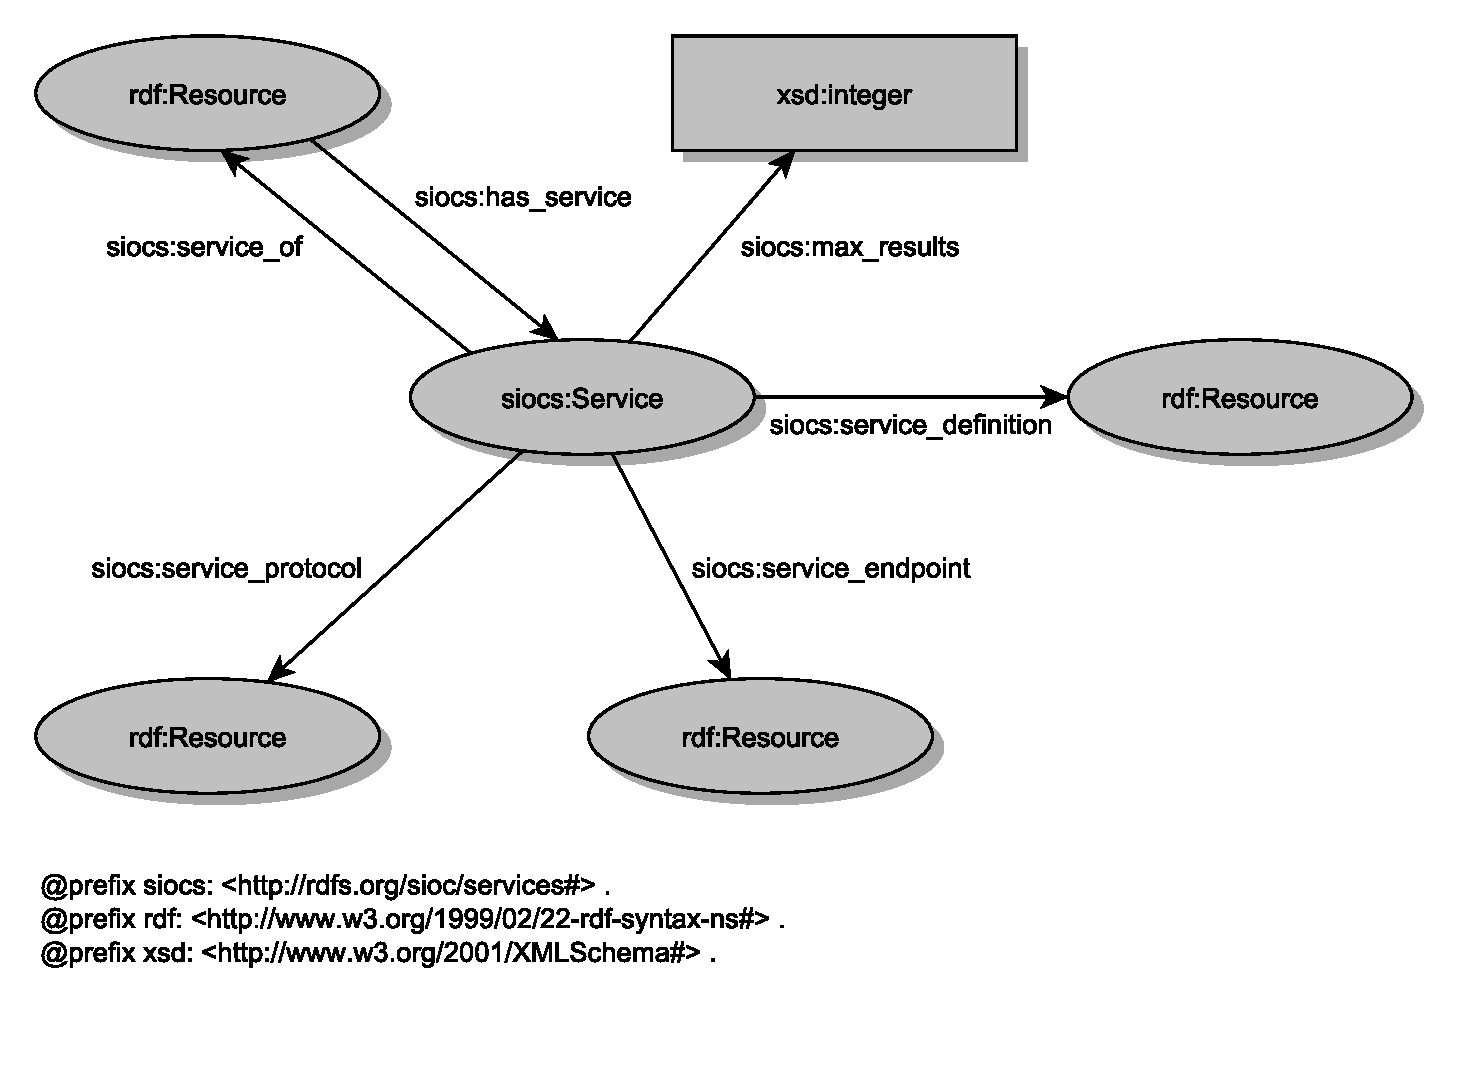
\includegraphics[
        width=0.7\textwidth,
        keepaspectratio=true
    ]{assets/images/sioc_services_ontology}
    \caption{SIOC Services Module}
    \label{fig:uebersicht_sioc_services}
\end{figure}

% subsection services (end)

\subsection{Benutzerdaten} % (fold)
\label{sub:benutzerdaten}

Soll ein Beitrag eines Benutzers von Google+ nach Facebook synchronisiert werden und es so aussehen, als hat er diesen Beitrag selbst auf Facebook geschrieben, sind gute Kenntnisse über alle Benutzerkonten dieser einen Person notwendig. Als erstes muss die Existenz dieser Person dem System bekannt sein. Hierzu kann diese durch die Klasse \texttt{Person} aus der FOAF Ontologie dargestellt werden. Für ein einzelnes Benutzerkonto wurde in SIOC die Klasse \texttt{UserAccount} definiert. Da \texttt{UserAccount} eine Unterklasse von \texttt{OnlineAccount} aus FOAF ist, kann diese über die Eigenschaft \texttt{foaf:account} beziehungsweise \texttt{sioc:account\_of} mit einer Person verbunden werden. Da es wichtig ist zu wissen zu welcher Webseiten ein Benutzerkonto gehört, wird der \texttt{UserAccount} mit einem Objekt der Klasse \texttt{Service} über die Eigenschaft \texttt{siocs:has\_service}
/\texttt{siocs:service\_of} zusammengebracht. Diese Verbindung ist für manche APIs besonders bedeutend, da in dem Serviceobjekt relevante Daten für den Zugriff darauf enthalten sind. Nun kann es vorkommen, dass eine Person private und geschäftliche Benutzerkonten besitzt. Um nicht private Beiträge auf Webseite A mit dem geschäftlichen Benutzerkonto auf Webseite B zu schreiben, muss ein Mapping zwischen den verschiedenen Benutzerkonten festgelegt werden. Dieses Mapping kann über ein in der \enquote{\nameref{sec:socc_connector_config_ontologie}} definierte Eigenschaft \texttt{mapped\_to} realisiert werden. Diese Eigenschaft ist bijektiv, also jedes Benutzerkonto maximal auf ein anderes Konto gemappt werden darf. Ebenso gilt, falls Benutzerkonto A mit Benutzerkonto B verbunden ist, ebenfalls B nach A gemappt wird. Abbildung \ref{fig:usermanagement} zeigt den zusammenhang zwischen der Klasse \texttt{Person}, \texttt{UserAccount} und \texttt{Service} sowie der Eigenschaft \texttt{mapped\_to} noch einmal graphisch an einem Beispiel.

\begin{figure}[ht]
    \centering
    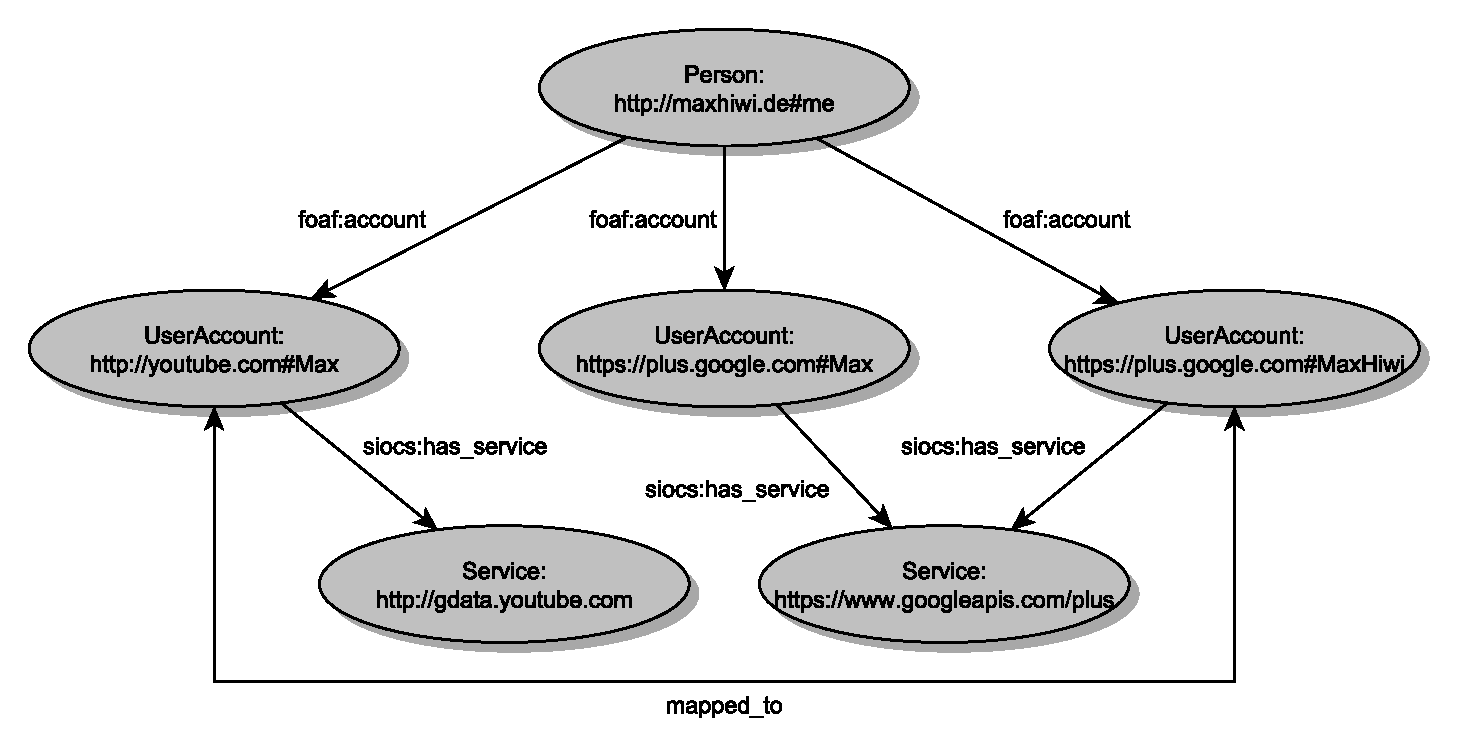
\includegraphics[
        width=\textwidth,
        keepaspectratio=true,]
    {assets/images/usermanagement}
    \caption{Zusammenhang von Person, UserAccount und Service. Die inversen Eigenschaften \texttt{sioc:account\_of} und \texttt{siocs:service\_of} wurden zu einer besseren Übersicht weggelassen}
    \label{fig:usermanagement}
\end{figure}

% subsubsection benutzerdaten (end)

\subsection{Authentifizierung} % (fold)
\label{sub:authentifizierung}

Die Ontologien FOAF und SIOC sind hervorragend für die Abbildung von sozialen Netzwerken und Diskussionen, jedoch ist es mit ihnen nicht möglich Daten zur Authentifizierung (Feststellen ob jemand der ist, den er vorgibt zu sein). Wegen dem Schutz der Privatsphäre ist dies verständlich, jedoch um stellvertretend für einen Benutzer Beiträge zu schreiben, ist es wichtig Zugriff auf diese Daten zuhaben und sie einem Benutzerkonto zuordnen zu können. Zuerst muss dazu aber festgestellt werden, welche verschiedenen Mechanismen es zum Anmelden ein solches Konto existieren.

\begin{description}
    \item[Username/Passwort] ist wohl eine der ersten und häufigsten Mechanismen, um den Zugriff sensibler Daten vor Dritten zu schützen. Das in Abschnitt \ref{sub:moodle_connector} beschriebene LMS Moodle, setzt zum Beispiel den Username und Password eines angemeldeten Benutzers zu Authentifizierung ein.
    
    \item[OAuth]\footnote{OAuth Webseite: \url{http://oauth.net/}} stellt heutzutage den Standard der verwendeten Authentifizierungsmechanismen für hauptsächlich webbasierte API dar. Benutzer können so temporär Programmen den Zugriff auf ihre Daten erlauben und später wieder verbieten. Der aktuelle Standard stellt OAuth 2.0 dar und wird in dieser Version von den größten Seitenbetreibern wie Google, Facebook oder Microsoft eingesetzt\footnote{OAuth Versionen im Einsatz: \url{http://en.wikipedia.org/wiki/OAuth\#List\_of\_OAuth\_service\_providers}}. Insgesamt sind für die Nutzung von OAuth vier Parameter wichtig. Für das Programm, dass Zugriff erhalten möchte sind die Parameter \emph{client\_id} und \emph{client\_secret} (Siehe \cite{rfc6749}[S.\,8]). Sie weisen das Programm als autorisiert für die Benutzung der Schnittstelle aus. Soll nun beim Aufrufer einer von OAuth geschützten Funktion belegt werden ist ein sogenannter Accesstoken nötig (Siehe \cite{rfc6749}[S.\,9]). Da dieser Accesstoken in der Regel nur eine bestimmte Zeit gültig ist, wird je nach Implementierung des Standards noch ein Refreshtoken mitgeliefert. Mit diesem Refreshtoken ist das Programm in der Lage ohne Zutun des Benutzers einen abgelaufen Accesstoken wieder zu aktivieren. Dies kann beliebig oft wiederholt werden, bis der Benutzer beide Token für ungültig erklärt.
    \todo[inline]{vll. noch OAuth 1.0(a) einbauen}
    
    \item[API Schlüssel] sind eine dritte Möglichkeit Programmen Zugriff auf eine API zu gewähren. Der API Schlüssel entspricht ungefähr einer Kombination von client\_id und client\_secret von OAuth. Dieser Schlüssel schaltet in der Regel nicht den Zugriff auf persönliche Daten von Benutzer frei. Hier ist noch ein weiterer Mechanismus wie die Verwendung von einem Usernamen und Passwort nötig. Die in Abschnitt \ref{sub:youtube_connector}  beschriebene Google Youtube API hierzu ein gutes Beispiel.
\end{description}

\begin{figure}[ht]
    \centering
    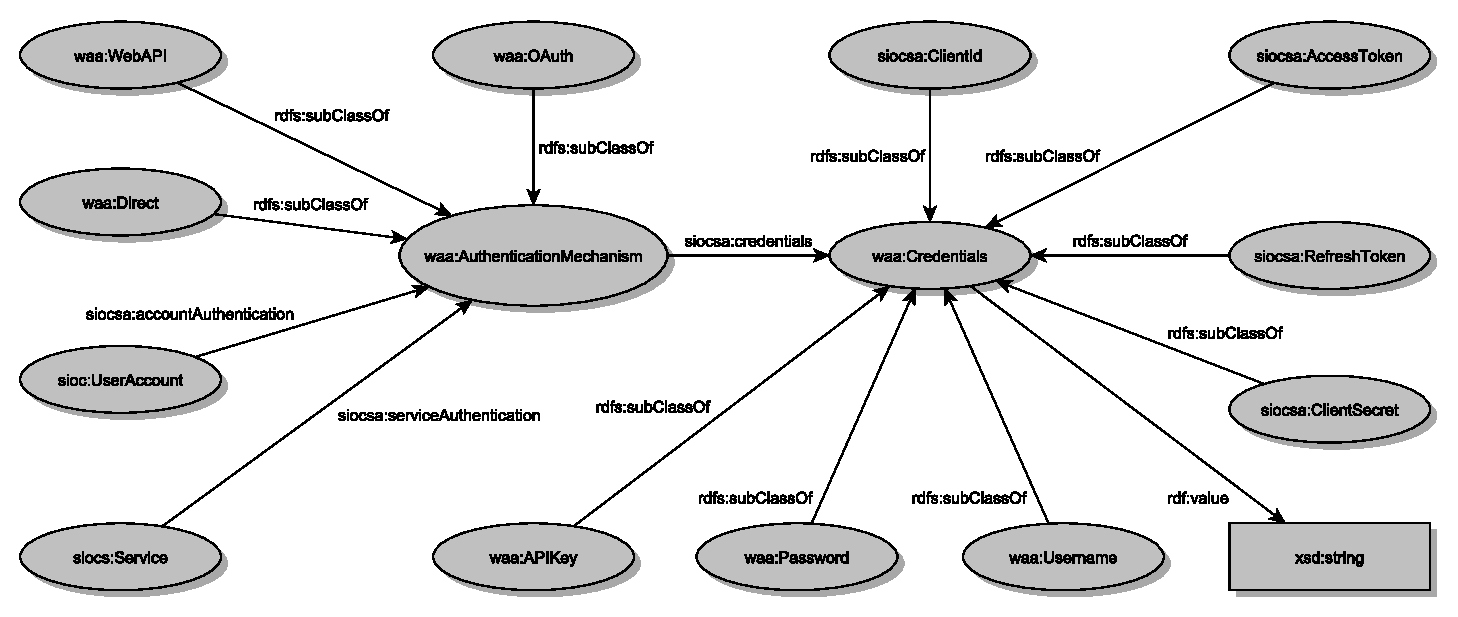
\includegraphics[
        width=\textwidth,
        keepaspectratio=true]
    {assets/images/sioc_services_authentication}
    \caption{SIOC Services Authentication Ontology}
    \label{fig:uebersicht_sioc_services_authentication}
\end{figure}

Neben diesen drei Mechanismen wäre noch der Vollständigkeit halber die HTTP-Authentifizierung zu nennen. Hierbei handelt es ich um eine Form des Username/Passwort Verfahrens, welches auf dem HTTP Protokoll aufsetzt. Für einfachen Webseiten ist dies ein unkomplizierte Art die Datei vor fremden Zugriffen zu schützten. Für aktuelle öffentliche APIs ist diese Form der Authentifizierung nicht mehr Stand der Technik.

Die Suche nach einer bestehen Ontologie, welche zusammen mit SIOC verwendet werden könnte, gestaltete sich als sehr schwierig. Ein Großteil der Ontologien in diese Richtung befasst sich eher mit dem Thema der Autorisierung wie zum Beispiel die \emph{Web Access Control List} \cite{Hollenbach2009} mit Zugriffssteuerungsliste. Eine Ausnahme stellt die \emph{Authentication Ontology}\footnote{Authentication Ontology: \url{http://omnivoke.kmi.open.ac.uk/authentication/}} des \emph{OmniVoke}\footnote{OmniVoke: \url{http://omnivoke.kmi.open.ac.uk/framework/}} Frameworks dar. Die Art der Authentifizierung wird darin durch die Klasse \texttt{AuthenticationMechanism} modelliert. Unterklassen für die wichtigsten Mechanismen wie \texttt{OAuth}, \texttt{WebAPI}s und Username/Password (dort \texttt{Direct} genannt) sind vorhanden. Jedem AuthenticationMechanism Objekt können dann sogenannte \texttt{Credentials} (engl. für Anmeldedaten) angehängt werden.

Das einzige Manko an dieser Ontologie war das Fehlen von Credentials für OAuth in der Version 2.0. Im einzelnen waren dies Klassen für clien\_id, client\_secret sowie für Access- und Refreshtoken. Um auch diese OAuth Version unterstützen zu können, wurden hierfür die Klassen ClientId, ClientSecret, AccessToken und RefreshToken als Unterklassen von Credentials abgeleitet. Als Letztes musste noch eine Verbindung zwischen Authentication Ontology und SIOC hergestellt werden. Zum Einen war eine Erweiterung der Klasse UserAccount notwendig, so dass die Anmeldedaten der Benutzer zur Verfügung standen. Zum Anderen werden Daten wie ein API Schlüssen von einen Service benötigt, die von denen der Benutzer unabhängig sind. Für die Klasse UserAccount wurde die Eigenschaft \texttt{accountAuthentication} geschaffen. Diese erwartet als Subjekt einen UserAccount und als Objekt ein AuthenticationMechanism, welcher dann die Credentials enthält. Für die Klasse Service existiert das Äquivalent \texttt{serviceAuthentication}. 

Diese Erweiterungen (Präfix \emph{siocsa:}) und die übernommenen Teile der Authentication Ontology wurden danach im \emph{SIOC Services Authentication Module} zusammengefasst. Graphisch ist sie in Abbildung \ref{fig:uebersicht_sioc_services_authentication} und im Anhang \ref{sec:sioc_services_authentication_module} als OWL Schema zu sehen. 

% subsection authorization (end)

\subsection{Autorisierung} % (fold)
\label{sub:autorisierung}

Da für viele Menschen im Internet ihre Privatsphäre und nicht wollen, dass ohne ihr Wissen Informationen von ihnen weitergegeben werden, ist es wichtig von den Benutzern die Erlaubnis zu holen Beiträge weiter zu leiten. Ein verbreitetes Mittel für eine solche Zugriffssteuerung sind Access Control Lists (ACL) (engl. für Zugriffsteuerungsliste). Die anderen nur einen begrenzten Zugriff auf eine feste Ressource gewähren. Für den Einsatz in dieser Arbeit wurde die Basic Access Control Ontologie \cite{Hollenbach2009,wiki:wacl} ausgewählt (Im Folgenden nur als ACL bezeichnet). Der Hauptgrund lag darin, dass sie auf FOAF aufbaut und sich so einfach integrieren ließ.

\begin{figure}[ht]
    \centering
    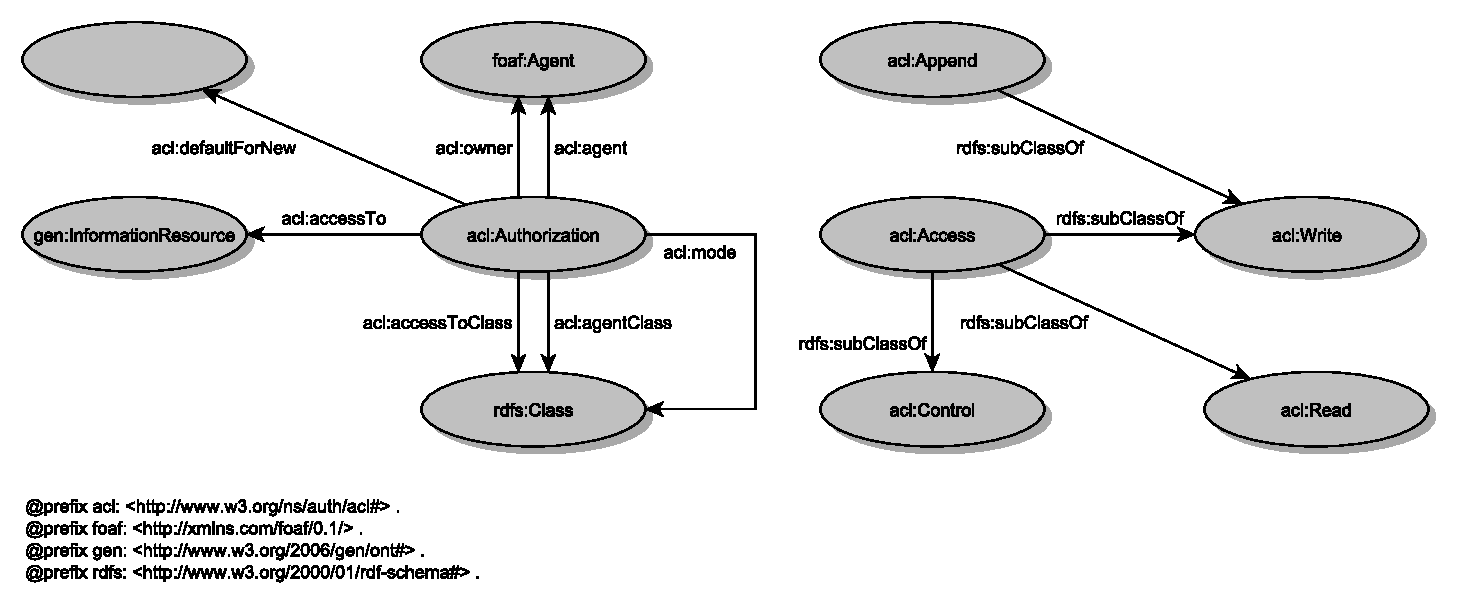
\includegraphics[
        width=\textwidth,
        keepaspectratio=true]
        {assets/images/w3c_web_acl}
    \caption{Basic Access Control Ontologie}
    \label{fig:w3c_web_acl}
\end{figure}

Die ACL stellt die Klasse \texttt{acl:Access} für die Abbildung eines Zugriffrechts auf eine Ressource zur Verfügung. Von dieser Klasse werden einzelne Rechte wie \texttt{acl:Read} für das Lesen und \texttt{acl:Write} für das Schreiben abgeleitet. Nebenbei existieren noch Ableitungen \texttt{acl:Control} zum Ausführen und \texttt{acl:Append} zum Anfügen von Inhalten. Diese sind für diese Arbeit aber nicht von Bedeutung.

Die eigentliche Regel für die ACL besteht aus der Klasse \texttt{acl:Authorization}. Der Besitzer dieser Regel wird durch die Eigenschaft \texttt{alc:owner} festgelegt. Der Besitzer ist im Fall von SOCC  ein Objekt der Klasse Person, wie in Abschnitt \ref{sub:benutzerdaten} \enquote{\nameref{sub:benutzerdaten}} beschrieben, da diese eine Unterklasse von der ACL geforderten \texttt{foaf:Agent} ist. Mittels \texttt{acl:agent} kann signalisiert werden, dass diese Regel nur für eine bestimmte Person/Agenten gilt. Das selbe gilt für \texttt{acl:agentClass}, wobei hier eine bestimmte Klasse gemeint ist. Soll zum Beispiel ein öffentlicher Zugriff definiert werden, wird \texttt{foaf:Agent} eingesetzt \cite[\enquote{Public Access}]{wiki:wacl}. Innerhalb von SOCC werden nur Regel angewendet, die einen solchen öffentlichen Zugriff erlauben. Die eigentlichen Rechte werden über die Eigenschaft \texttt{acl:mode} festgelegt. Erlaubt ist die Angabe jeder beliebigen Klasse, SOCC testet aber nur auf die Klassen \texttt{acl:Read} und \texttt{acl:Write} zum Lesen und Schreiben von Beiträten. Auf welche Ressource sich ein Regel letztendlich bezieht, wird über die Eigenschaft \texttt{acl:accessTo} geregelt. Die Angabe von \enquote{http://www.facebook.com} würde sich für SOCC zum Beispiel auf alle Beiträge des Besitzers auf Facebook beziehen, \enquote{https://canvas.instructure.com/courses/798152} dahingegen nur auf alle Beiträge innerhalb eines Canvas Kurses. Für einen Zugriff auf alle Beiträge prüft SOCC ob die Eigenschaft \texttt{acl:accessToClass} auf die Klasse \texttt{sioc:Post} verweist. So müsste nicht jede einzelne Seite angegeben werden.

% access und accessClass fehlen

Das Listing \ref{lst:acl_beispiel} zeigt ein Beispiel wie ein ACL Regel aussehen könnte. Der Besitzer dieser Regel wird durch die URI \texttt{http:/example.org\#john} beschrieben (Zeile 6). Diese Person erlaubt nun öffentlichen Zugriff (Zeile 7) all all seine Beiträge (Zeile 8). Dieser Zugriff kann sowohl lesend als auch schreibend erfolgen (Zeile 9).

\begin{lstlisting}[
    caption={ACL Beispiel}\label{lst:acl_beispiel},
    captionpos=t]
@prefix sioc: <http://rdfs.org/sioc/ns#> .
@prefix foaf: <http://xmlns.com/foaf/0.1/>
@prefix acl: <http://www.w3.org/ns/auth/acl#> .

[] a acl:Authorization;
    acl:owner <http:/example.org#john>;
    acl:agentClass foaf:Agent;
    acl:accessToClass sioc:Post;
    acl:mode acl:Read, acl:Write .
\end{lstlisting}

% subsection autorisierung (end)

% section konfiguration (end)

\section{Design eines Connectors} % (fold)
\label{sec:design_eines_connectors}

\todo[inline]{Einleitung für design schreiben}

\begin{figure}[ht]
    \centering
    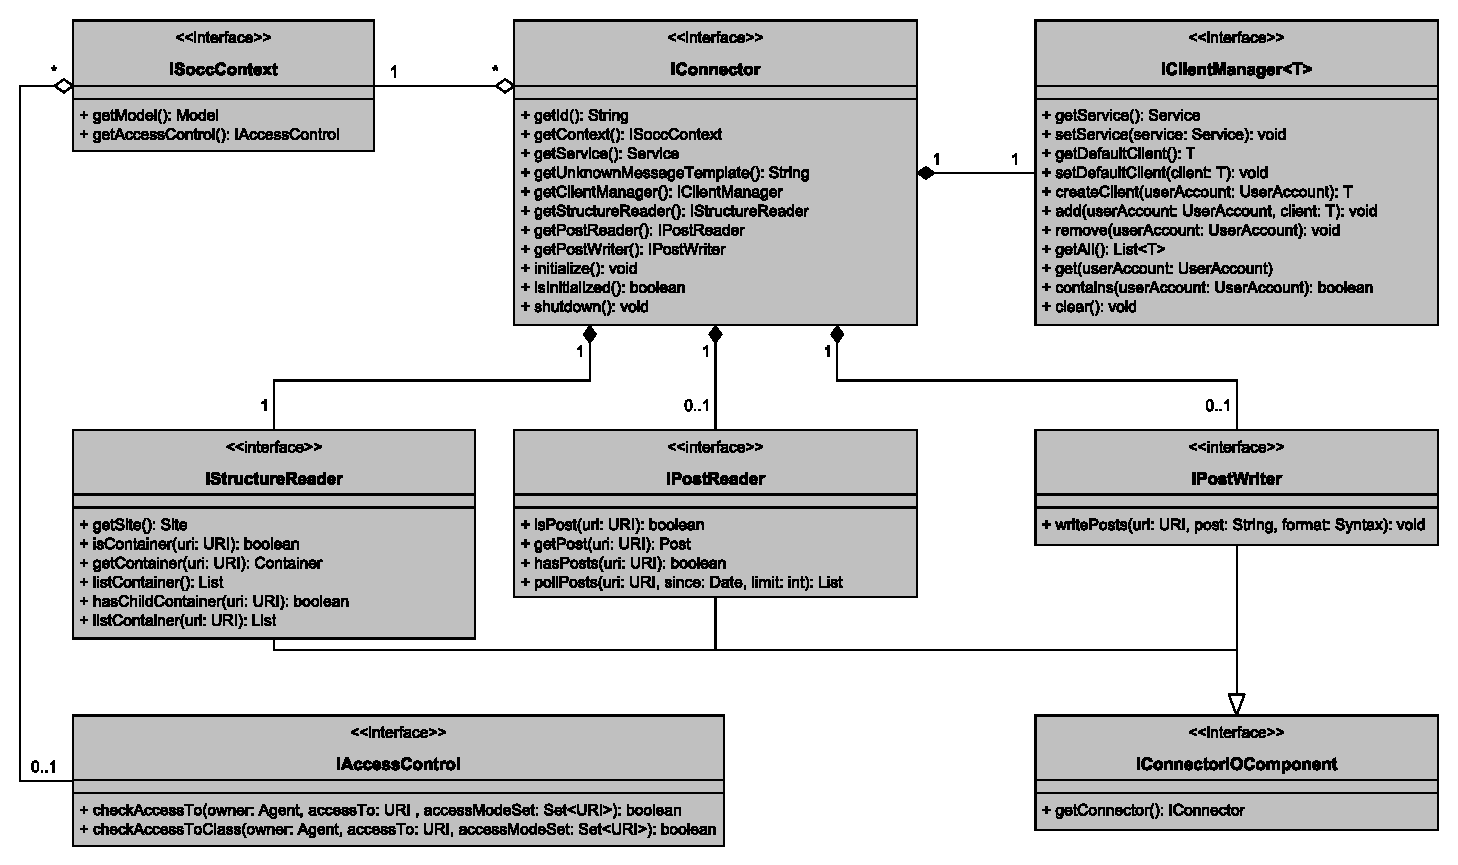
\includegraphics[
        scale=0.95,
        keepaspectratio=true,
        angle=90]
    {assets/images/socc_uml_classdiagram}
    \caption{UML Klassendiagramm eines Connectors}
    \label{fig:connecotr_uml_classdiagram}
\end{figure}

% subsection design_eines_connectors (end)

\subsection{SOCC Context} % (fold)
\label{sub:socc_context}

\begin{wrapfigure}{r}{6cm}
    \centering
    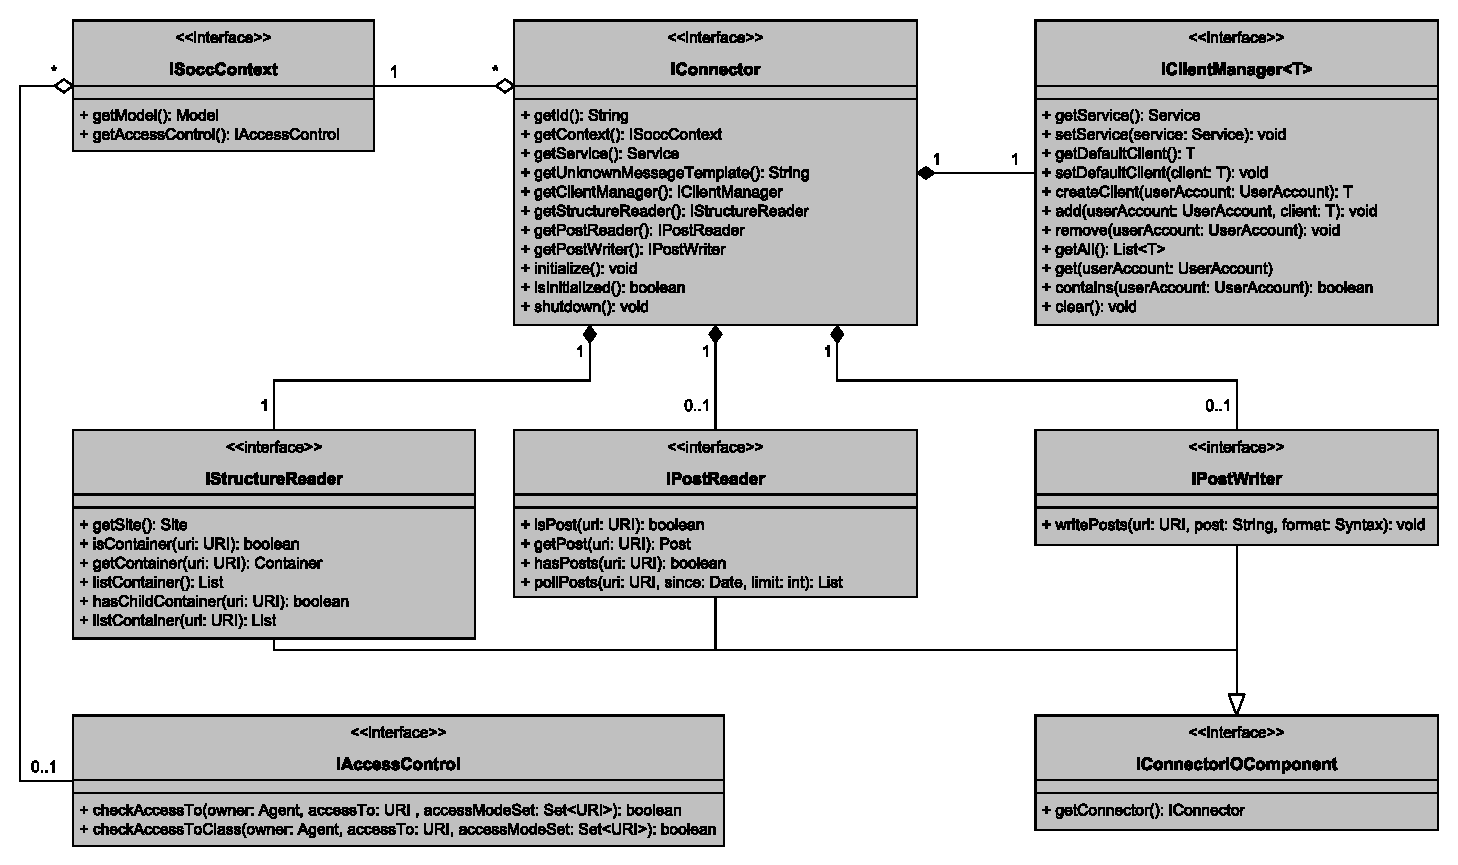
\includegraphics[
        width=6cm,
        keepaspectratio=true,
        clip=true,
        trim= 35 340 520 9]
    {assets/images/socc_uml_classdiagram}
    \caption{SOCC Context}
    \label{fig:uml_socc_context}
\end{wrapfigure}

Der Kontext eines Connectors beschreibt die Umgebung innerhalb dem er seine Arbeit verrichtet. Im aktuellen Status erhält der Connector zum einen Zugriff auf ein außenstehendes Model (TripleStore), das wichtige Daten für den Betrieb und enthält oder abgelegt werden können. Eine Referenz auf dieses Model erhält der Connector über den Aufruf der Funktion \texttt{getModel()}. Durch die Methode \texttt{getAccessControl()} kann der Connector über die im nächsten Abschnitt beschriebene AccessControl Schnittstelle auf die Information für die Zugriffssteuerung für das Lesen und Schreiben von Beiträgen. 

% subsubsection socc_context (end)

\subsection{AccessControl} % (fold)
\label{sub:accesscontrol}

\begin{wrapfigure}{r}{12cm}
    \centering
    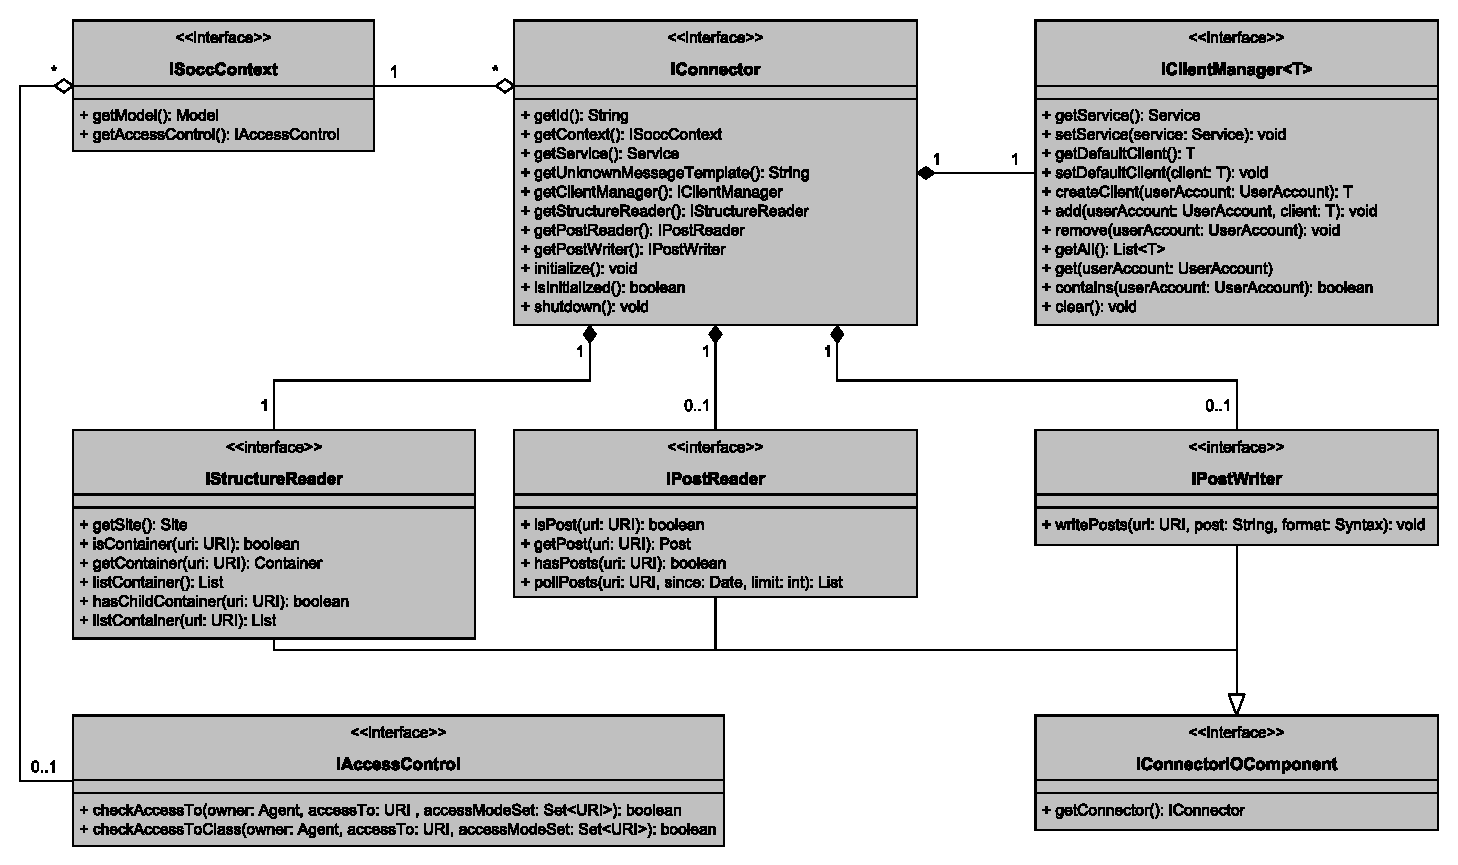
\includegraphics[
        width=12cm,
        keepaspectratio=true,
        clip=true,
        trim= 35 8 350 340]
    {assets/images/socc_uml_classdiagram}
    \caption{AccessControl}
    \label{fig:uml_accesscontrol}
\end{wrapfigure}

Die AccessControl Schnittstelle ist sehr einfach gehalten und dient für den Zugriff auf die in Abschnitt \ref{sub:authentifizierung} \enquote{Autorisierung} beschriebene ACL. Die Methode \texttt{checkAccessTo(\dots)} prüft, ob der Zugriff auf eine Ressource mit allen übergebenen Zugriffsmodi erlaubt ist. Die andere Methode \texttt{checkAccessToClass} ist zur Überprüfung, die die Rechte für den Zugriff auf eine komplette Klasse von Ressourcen. 

% subsubsection accesscontrol (end)

\subsection{ClientManager} % (fold)
\label{sub:clientmanager}

\begin{wrapfigure}{r}{9cm}
    \centering
    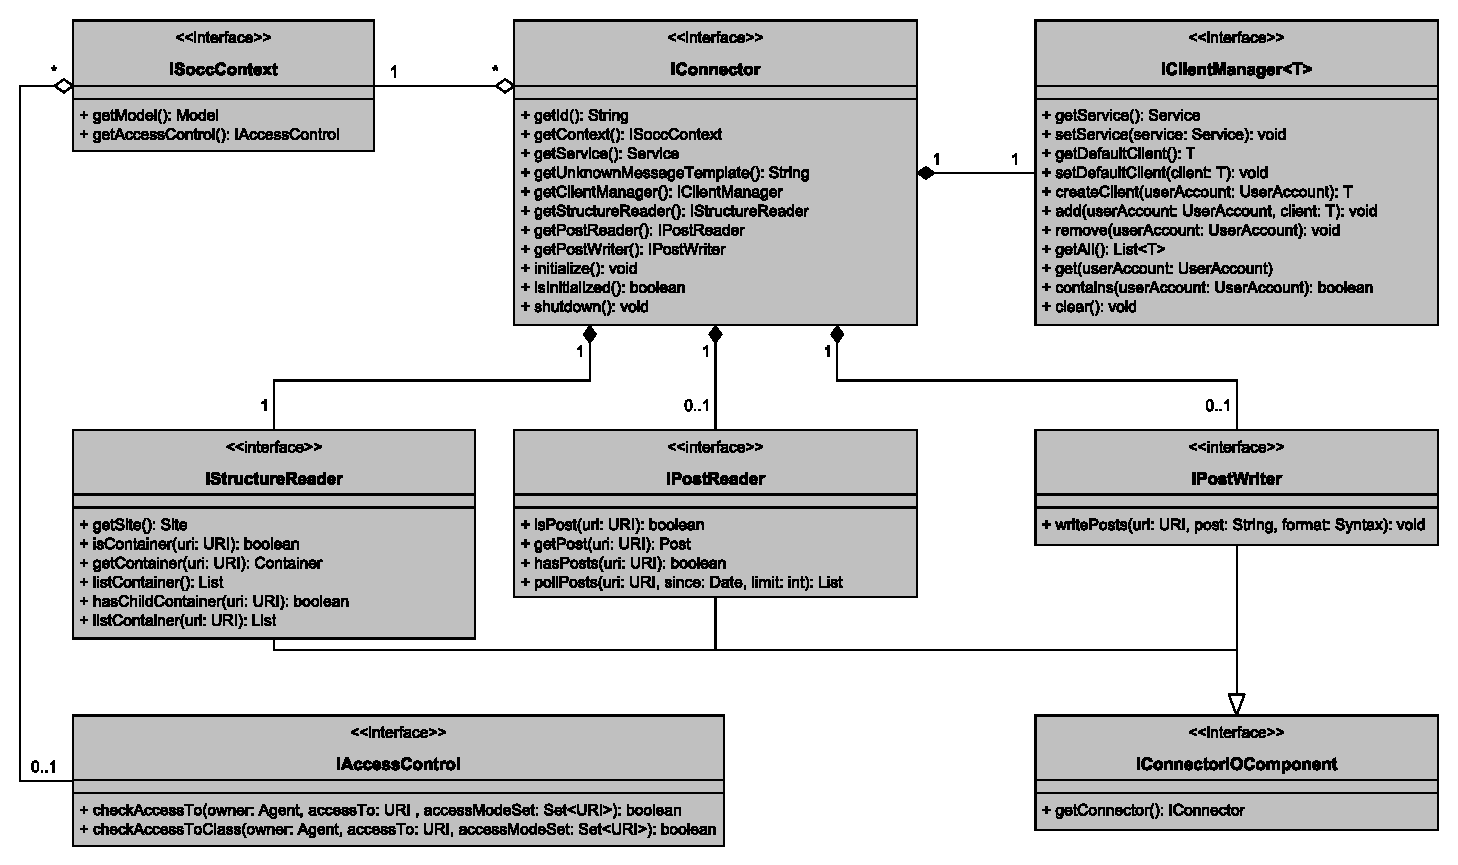
\includegraphics[
        width=9cm,
        keepaspectratio=true,
        clip=true,
        trim= 497 257 9 9]
    {assets/images/socc_uml_classdiagram}
    \caption{ClientManager}
    \label{fig:uml_clientmanager}
\end{wrapfigure}

Der Zugriff auf eine API innerhalb eines Programms erfolgt in der Regel über eine sogenanntes Clientobjekt (kurz Client). Dieser Client erlaubt es mit den Anmeldedaten oder den Accesstoken für ein Benutzerkonto auf die Funktionen der API über verschiedene Methoden zu zugreifen. Da ein Client immer nur mit einem Benutzerkonto verknüpft ist und von diesen eine große Anzahl verwaltet werden müssen, enthält jeder Connector einen ClientManager. Der interne Aufbau eines Client ist dabei stark von der verwendeten API abhängig und arbeitet mit dem Connector zusammen für den er geschrieben wurde. Für alle benutzerunabhängigen Daten erhält der ClientManager ein wie Abschnitt \ref{sub:services} beschriebenes Serviceobjekt. Ein neuer Client kann dann durch den Aufruf der Methode \texttt{createClient(\dots)} erstellt werden. Als Parameter wird der Methode ein Benutzerkonto in Form eines SIOC UserAccounts übergeben. Sind alle erforderlichen Autorisierung- und Authentifizierungsinformation aus Abschnitt \ref{sub:authentifizierung} vorhanden, wird ein neuer Client erzeugt und zurück gegeben. Dieser Client wird aber dadurch nicht automatisch vom ClientManager verwaltet. Hierzu muss der im vorherigen erzeugte Client durch den Aufruf von \texttt{add(userAccount: UserAccount, client: T )} dauerhaft mit den angegeben UserAccount verknüpft und intern gespeichert. Wichtig ist hierbei, dass die Eigenschaften \texttt{accountName} und \texttt{accountServiceHomepage} des UserAccount Objekts gesetzt sind. Aus diesen wird ein eindeutiger Schlüssel generiert der zur Zuordnung von UserAccount und Client innerhalb des ClientManagers dient. Des weiteren stehen noch Methoden \texttt{remove(userAccount: UserAccount)} zum Entfernen und \texttt{get(userAccount: UserAccount)} Holen von Clients, sowie \texttt{contains(userAccount: UserAccount)} für Tests ob ein Client zu einem UserAccount existiert. Sollen zum Beispiel am Ende der Laufzeit des Programms alle erzeugten Clients auf einmal abgemeldet und gelöscht werden, kann dies über die Methode \texttt{clear()} erfolgen. Der ClientManager verwaltet ebenfalls den Client für den in Abschnitt \ref{sub:connector_config_ontologie} angesprochenen Defaultuser. Dieser Defaultclient genannte Client kann über die Methode  \texttt{setDefaultClient(client: T)} gesetzt und durch \texttt{getDefaultClient()} jederzeit wieder abgerufen werden. 

% subsubsection clientmanager (end)

\subsection{StructureReader} % (fold)
\label{sub:structurereader}

\begin{wrapfigure}[10]{r}{9cm}
    \centering
    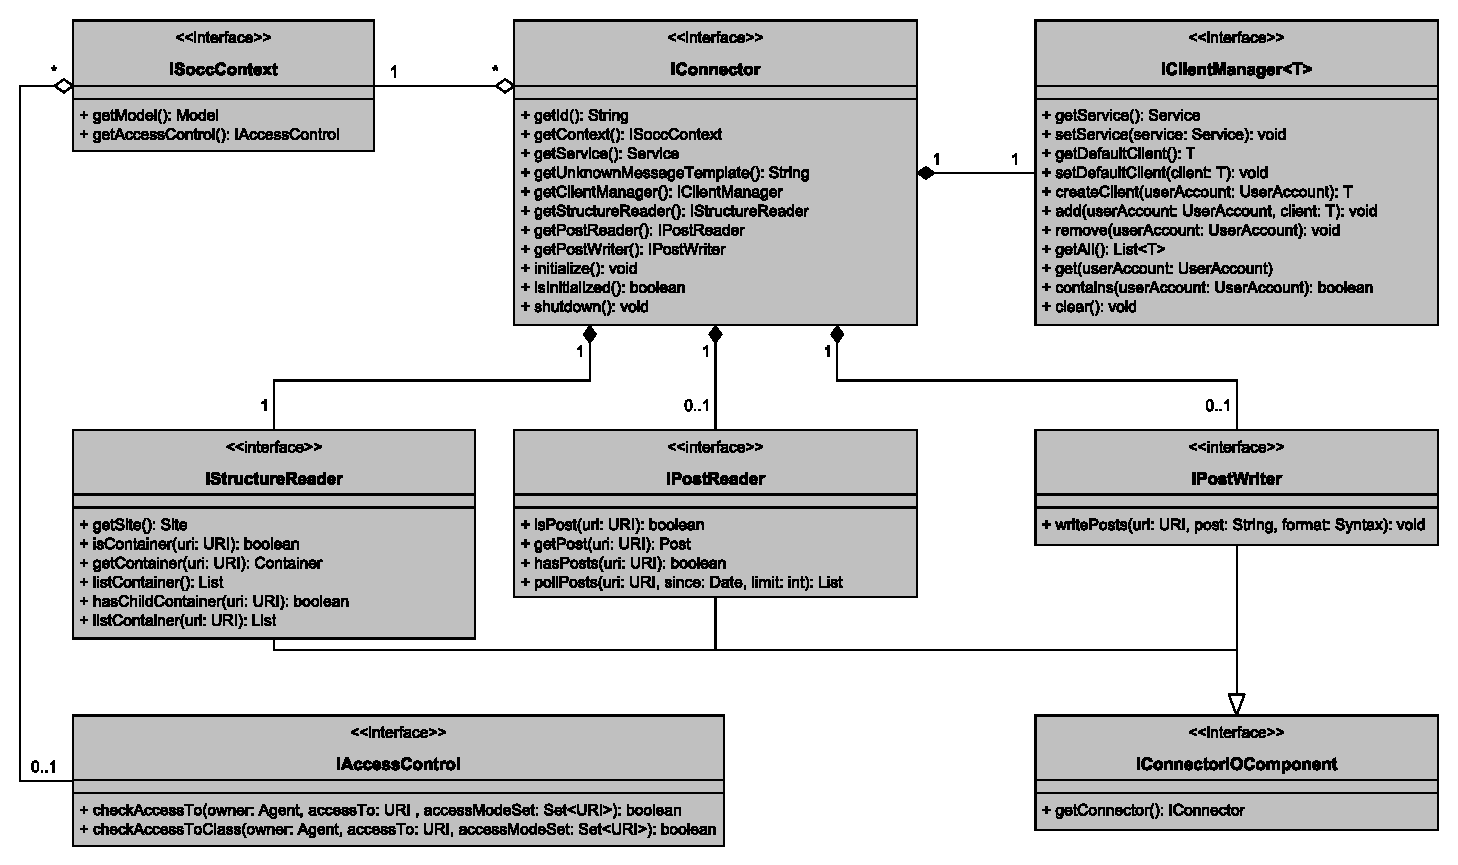
\includegraphics[
        width=9cm,
        keepaspectratio=true,
        clip=true,
        trim= 20 109 456 206]
    {assets/images/socc_uml_classdiagram}
    \caption{StructurReader}
    \label{fig:uml_structure_reader}
\end{wrapfigure}
Um auf Informationen über die Struktur von Foren, sozialen Netzwerken und so weiter im SIOC Format zugreifen zu können, implementiert jeder Connector dazu einen StructureReader. Die Struktur lässt sich, wie im Abschnitt \ref{ssub:semantically_interlinked_online_communities} vorgestellt, durch die SIOC Klassen \emph{Site} und \emph{Container} (und Unterklassen davon) beschrieben. Um auf diese Struktur zugreifen zu können, enthält die StructureReader Schnittstelle mehrere Methoden (Siehe Abbildung \ref{fig:uml_structure_reader}). \wrapfill

\begin{description}
    \item[\texttt{getSite()}] ist eine Methode, welche die Beschreibung einer Seite (Forum, Blog, soziales Netzwerk) als SIOC Site Objekt zurücklieft. Dies wird relativ häufig um die Zugehörigkeit einiger Objekte durch einen Link zu dieser Seite zu verdeutlichen. Dies kann bei einigen APIs nützlich sein, da dort manchmal keine Information zum \emph{Container} eines Beitrags mitgeliefert werden, über den man sonst eine Beziehung zwischen Seite und Beitrag herstellen könnte.

    \item[\texttt{isContainer(uri: URI)}] wird zu Überprüfung verwendet, ob sich hinter einer URI ein potenzieller Container befindet. 

    \item[\texttt{getContainer(URI)}] ist dazu gedacht die Information eines einzelnen Containers erhalten der sich hinter eine URI verbirgt.

    \item[\texttt{listContainer(\dots)}] sind Methoden welche für den die Auflisten aller Container einer Seite zur Verfügung stehen. Die Methode ohne Parameter listet alle Container auf der ersten Ebene auf. Dies könnten zum Beispiel alle Kurse auf einen Canvas LMS Seite oder alle Gruppen auf Facebook sein. Die zweite Methode mit URI Parameter gibt eine Liste alle Container, welche den Container hinter der übergeben URI als Elternteil haben, zurück. Als Beispiel wären alle Themen innerhalb eines Forums zu nennen.

    \item[\texttt{hasChildContainer(uri: URI)}] überprüft ob der Container hinter einer URI überhaupt weitere Container als Kinder besitzt. Diese Methode wird dazu eingesetzt, um vorab zu testen, ob der Aufruf von \texttt{listContainer(URI)} das gewünschte Ergebnis liefert oder ein Fehler auftritt. 
\end{description}

% subsubsection structurereader (end)

\subsection{PostReader} % (fold)
\label{sub:postreader}

\begin{wrapfigure}{r}{9cm}
    \centering
    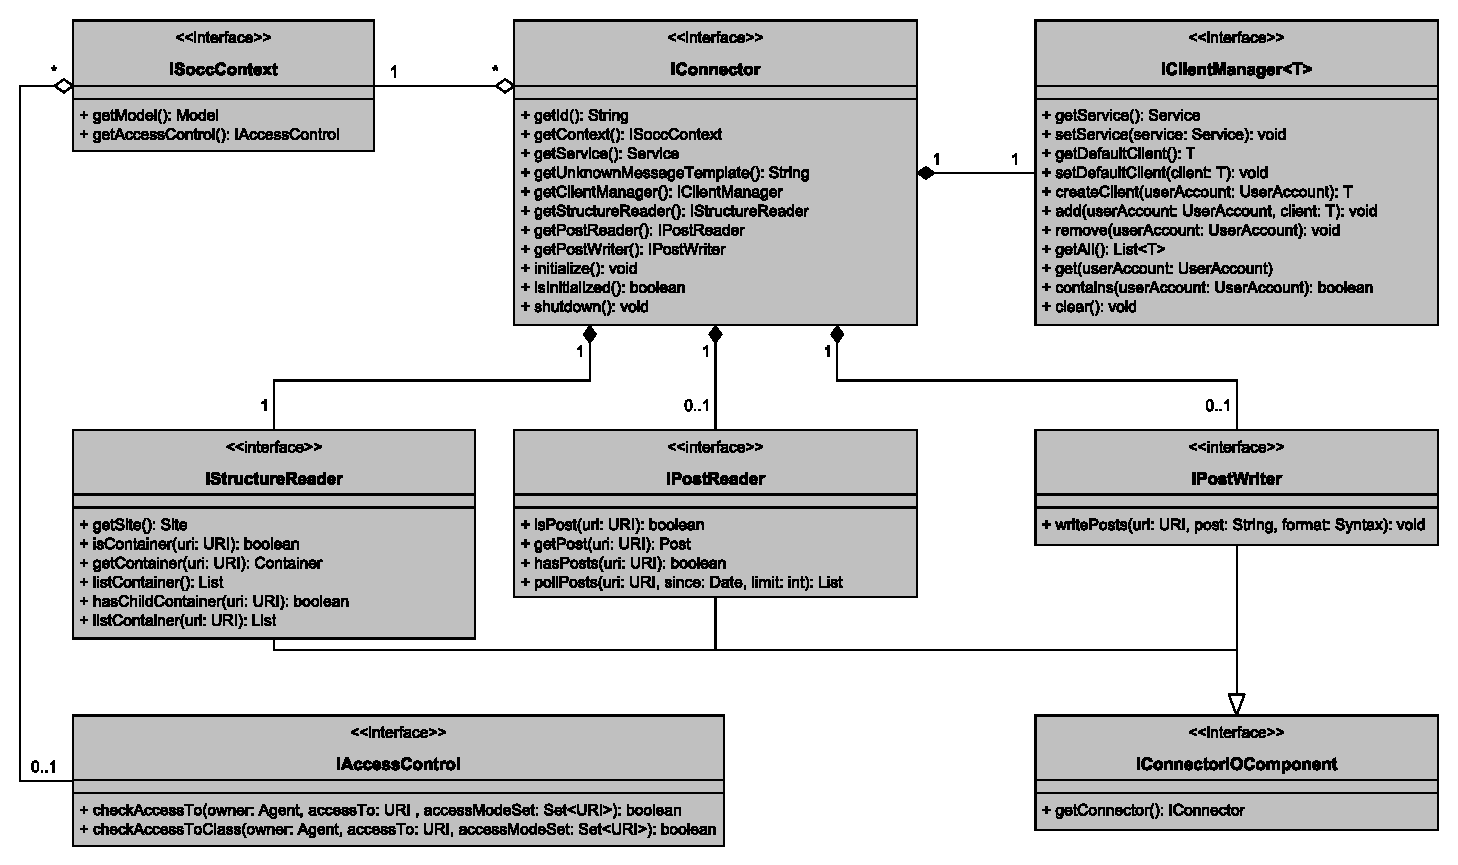
\includegraphics[
        width=9cm,
        keepaspectratio=true,
        clip=true,
        trim= 243 129 255 206]
    {assets/images/socc_uml_classdiagram}
    \caption{PostReader}
    \label{fig:uml_post_reader}
\end{wrapfigure}

Der \texttt{PostReader} dient als Schnittstelle für das Lesen geschriebener Beiträge innerhalb eines Containers oder der Kommentare auf einen anderen Beitrag. Er stellt nach außen hin Funktionen bereit mit denen entweder ein einzelner Beitrag oder alle Beiträge die bestimmte Kriterien erfüllen gelesen werden können. Bevor ein Beitrag zurück gegeben wird, müssen die Methoden prüfen, ob der Autor dieses Beitrag das Lesen dafür erlaubt hat. Falls nicht, wird der Beitrag aus der Ergebnisliste gelöscht oder ein Fehler ausgegeben. Die Funktionsweise der einzelnen Methoden ist wie folgt:

\begin{description}
    \item[\texttt{isPost(uri: URI)}] kann zur Überprüfung eingesetzt werden, ob sich hinter einer URI ein Beitrag befindet.

    \item[\texttt{getPost(uri: URI)}] ist dazu gedacht einen einzelnen Beitrag anhand seiner URI zu lesen. Sie liefert dann den Beitrag SIOC Post Objekt zurück beziehungsweise einen Fehler, falls der Beitrag nicht mit diesem Connector gelesen werden kann.

    \item[\texttt{hasPost(uri: URI)}] funktioniert ähnlich wie isPost, überprüft aber ob sich hinter der angegeben URI noch weitere Beiträge befinden. 

    \item[\texttt{pollPosts(uri: URI, since: Date, limit: int)}] ist eine Methode mit der alle Beiträge hinter eine URI liest und anhand der übergebenen Kriterien filtert.  Insgesamt erhält diese Methode drei Parameter. Der Erste ist eine URI die den Ort angibt von der alle Beiträge gelesen werden können. Mit dem zweiten Parameter kann ein Zeitpunkt angegeben werden, ab dem ein zu lesender Beitrag geschrieben sein muss. Zum Beispiel der Zeitpunkt als diese Methode das letzte mal aufgerufen wurde, um alle Beiträge die danach folgten zu lesen. Der letzte Parameter gibt eine obere Schranke an, wie viele Beiträge maximal pro Aufruf dieser Methode gelesen werden dürfen. 
\end{description}

% subsubsection postreader (end)

\subsection{PostWriter} % (fold)
\label{sub:postwriter}

In Abbildung \ref{fig:postwriter_sequenzdiagramm} ist ein Sequenzdiagramm der PostWriter Komponente zu sehen. Dort ist visualisiert, welche Schritte für das stellvertretende Schreiben von Beiträgen eines Benutzers unternommen werden müssen. Soll nun ein Beitrag in einer SOC geschrieben werden, wird die Methode \texttt{writePost(URI, String, Syntax)} mit dem Zielort als URI, dem Beitrag als serialisiertes RDF Objekt und dem verwendeten Serialisierungsformates aufgerufen. Begonnen wird damit, dass als erstes nach einem UserAccount für den Service des aktuellen Connectors des Beitragautors gesucht. Im Idealfall befindet sich für den UserAccount des Beitragsautors ein Link zu seiner FOAF Person und von ein weiterer Link zum UserAccount für den aktuellen Service. Mit diesem UserAccount kann dann vom ClientManager ein Clientobjekt für die verwendete API angefordert werden. Sollte die Suche negativ verlaufen, steht der Defaultclient zur Verfügung. Mit diesem Client, ob mit der des Autors oder dem Defaultclient, wird im letzten Schritt der Beitrag im von der API verwendeten Format in die SOC geschrieben.

\todo[inline]{unknownMessageTemplate und Watermark erwähnen}

\begin{figure}[ht]
    \centering
    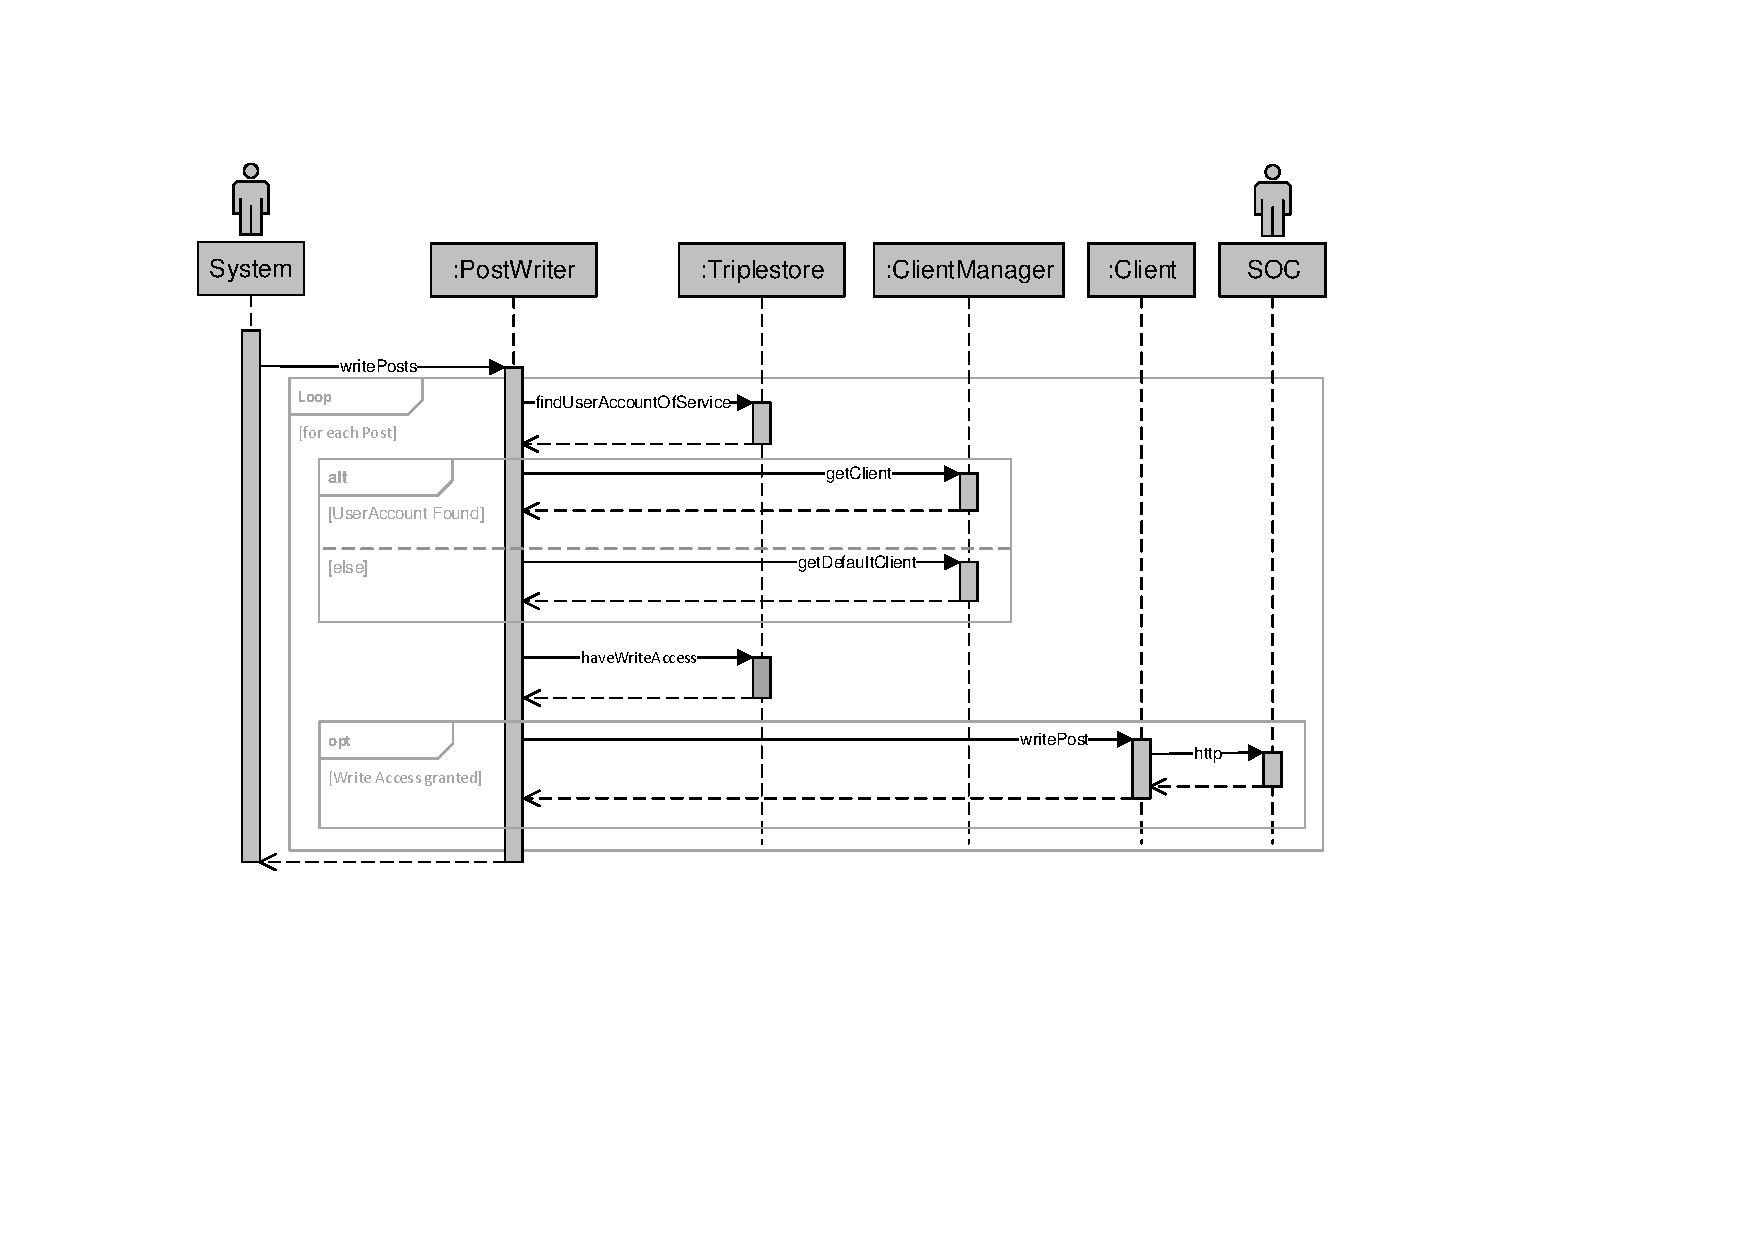
\includegraphics[
        width=\textwidth,
        keepaspectratio=true,
        clip=true,
        trim= 90 200 220 75]
    {assets/images/postwriter_sequencediagram}
    \caption{UML Sequenzdiagramm eines PostWriters}
    \label{fig:postwriter_sequenzdiagramm}
\end{figure}

% subsubsection postwriter (end)

% subsection connector_aufbau (end)

% section social_online_community_connectors (end)

\section{SOCC-Camel} % (fold)
\label{sec:socc_camel}

\emph{SOCC-Camel} ist eine Modul der SOCC für die Einbindung von Connectoren in das Apache Camel Framework. Durch dieses ist es sehr einfach möglich die gelesenen Beiträte von einer SOC in eine andere zu schreiben. Abbildung \ref{fig:uebersicht_socc_camel} zeigt SOCC-Camel als EIP-Diagramm. 

\begin{figure}[ht]
     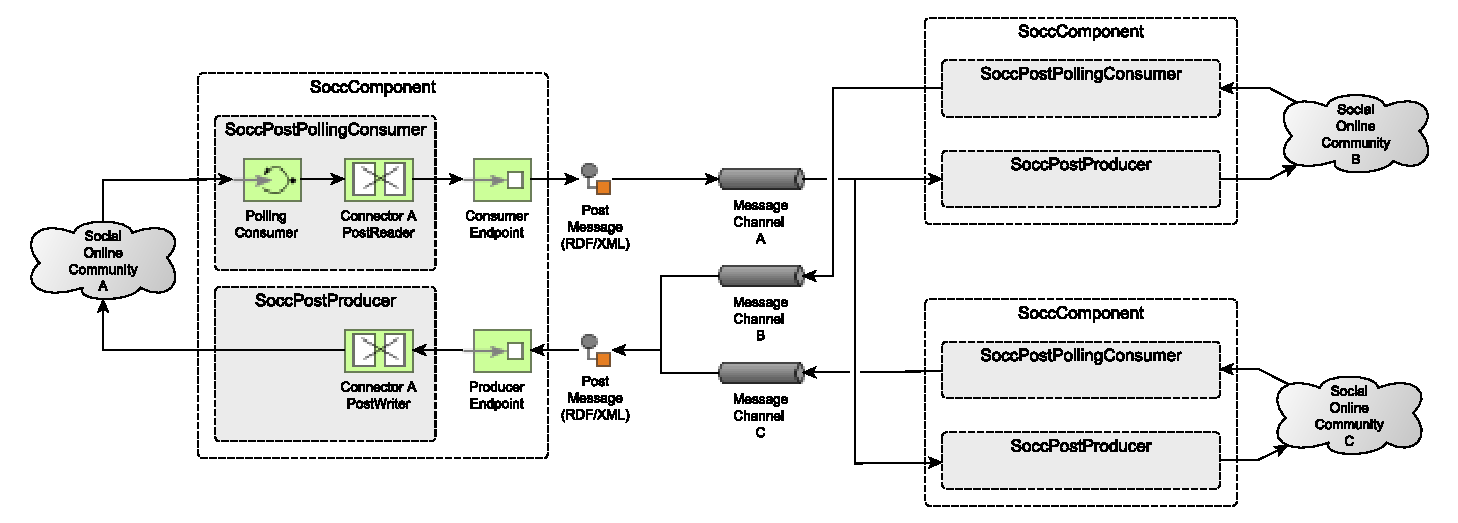
\includegraphics[
        width=\textwidth,
        keepaspectratio=true]
        {assets/images/socc_camel_overview}
    \caption{Übersicht des Socc-Camel Moduls in EIP-Notation}
    \label{fig:uebersicht_socc_camel}
\end{figure}

Hauptklasse dieses Modul ist die Klasse \texttt{SoccComponent} und ist für die Verwaltung von Connectoren und Erstellen der Endpoints für Apache Camel zuständig. Von dieser Klasse SoccComponent muss zuerst ein Objekt erzeugt und ein Objekt einer Klasse welche die Schnittstelle \texttt{ISoccContext} implementiert. Das das damit übergebende Model mit dem Triplestore sollte alle Daten für die Erstellung der später genutzten Connectoren und deren Betrieb enthalten. Also alle Daten die in Anschnitt \ref{sec:konfiguration} beschrieben sind. Das nun vorhandene SoccComponent Objekt wird dann unter einen frei wählbaren Namen in Apache Camel registriert. Nun kann wie in Abschnitt \ref{ssub:apache_camel} mit dieser Komponente eine Route erstellt werden. Die Konfigurationsuris habe dazu den folgenden Aufbau:

\begin{lstlisting}[
    caption={SOCC-Camel Konfigurations URI}\label{lst:socc_camel_uri},
    captionpos=t]
socc://{connectorId}?uri={targetUri}[&{options}...]
\end{lstlisting}

Der Anfang der URI mit \enquote{socc://} sagt Apache Camel, dass es für diesen Endpoint die Component benutzten soll, die unter dem Namen \enquote{socc}. Hier wäre dies eine der Klasse SoccComponent. Für den Platzhalte \enquote{\{connectorId\}} muss eine gültige ID eines Connectors sein, dessen Konfigurationsdaten im TripleStore. befinden. Über den URI Parameter \enquote{uri} wird dann die Quell- beziehungsweise Zieluri für den Connector angegeben. Im Falle, dass es sich um eine URI für den Startpunkt einer URI handelt, können am Ende noch weitere Parameter angehängt werden.

\subsection{SoccPostPollingConsumer} % (fold)
\label{sub:soccpostpollingconsumer}

Wird ein Endpoint mit der Absicht zum Lesen von Beiträgen erstellt, erzeugt die Klasse SoccComponent eine Objekt der Klasse \texttt{SoccPostPollingConsumer} und übergibt im die Parameter aus der verwendeten URI. Als zusätzliche Parameter für die URI können \texttt{delay} und \texttt{limit angegeben werden}. Da SoccPostPollingConsumer sich von der Klasse \texttt{ScheduledPollConsumer} ableitet, ist es über den Parameter \texttt{delay} möglich in periodischen Abständen Aufgaben abzuarbeiten. In diesen Fall das Lesen von neuen Beiträgen. Die Angabe erfolgt dabei in Millisekunden. Der Parameter \texttt{limit} entspricht dabei den gleichnamigen Argument der Methode \texttt{pollPosts} des PostReaders aus Abschnitt \ref{sub:postreader}. Das dort noch fehlende Argument \texttt{since}, für das Datum ab wann ein Beitrag als neu gilt, holt sich der SoccPostPollingConsumer aus den im TripleStore gespeicherten Daten. Zum Beispiel durch das Datum des zuletzt gelesenen Beitrags aus einen Thread oder das des letzten Kommentars. Alle neue gelesenen Beiträge werden am Ende in das RDF/XML serialisiert und als Nachricht an Apache Camel übergeben, welches es dann anhand der festgelegte Routen weiterleitet. Dass andere Komponenten diese Nachricht wieder korrekt de-serialisieren können, muss der Nachricht noch ein Header \enquote{Content-Type} mit dem MIME-Type\footnote{ Multipurpose Internet Mail Extension - Types: \url{http://tools.ietf.org/html/rfc2046}} vom RDF/XML \enquote{application/rdf+xml} mitgegeben werden

% subsection soccpostpollingconsumer (end)

\subsection{SoccPostProducer} % (fold)
\label{sub:soccpostproducer}

Der \texttt{SoccPostProducer} ist das Gegenstück zum SoccPostPollingConsumer er ist der Endpoint der zum Schreiben von Beiträgen zurück eine ein SOC von der SoccComponent erzeugt wird. Intern verwendet er die PostWriter Komponente des betreffenden Connetors und leitet den Inhalt der Nachricht an diese weiter. Außer der Angabe über die Zieluri erhält der SoccPostProducer keine weiteren Parameter über die Konfigurationsuri.

% subsection soccpostproducer (end)

% section socc_camel (end)

% chapter eigener_ansatz_social_online_community_connectors_socc_ (end)
